\documentclass[oneside]{VUMIFPSkursinis}
\usepackage{algorithmicx}
\usepackage{algorithm}
\usepackage{algpseudocode}
\usepackage{amsfonts}
\usepackage{float}
\usepackage{amsmath}
\usepackage{bm}
\usepackage{caption}
\usepackage{color}
\usepackage{float}
\usepackage{graphicx}
\usepackage{listings}
\usepackage{subfig}
\usepackage{tabularx}
\usepackage{wrapfig}
\newcolumntype{P}[1]{>{\centering\arraybackslash}p{#1}}
\usepackage[%  
    colorlinks=true,
    linkcolor=black
]{hyperref}
\university{Vilniaus universitetas}
\faculty{Matematikos ir informatikos fakultetas}
\department{Programų sistemų katedra}
\papertype{Laboratorinis darbas II}
\title{Automatinė ūkio valdymo sistema}
\titleineng{Automatic Farm Management System}
\status{2 kurso 3 grupės studentai}
\author{Matas Savickis}
\secondauthor{Justas Tvarijonas}  
\thirdauthor{Greta Pyrantaitė}   
\fourthauthor{Rytautas Kvašinskas}
\supervisor{Karolis Petrauskas, Doc., Dr.}
\date{Vilnius – \the\year}


\bibliography{bibliografija}

\begin{document}
\maketitle


\centering

 
\tableofcontents


\section{Įvadas}
\subsection{Tikslas}
Šiuo dokumentu siekiame detaliai perteikti Automatinės ūkio valdymo sistemos aprašą. Dokumente pateikti sistemos tikslai, jų įgyvendinimas, sąsajos su išore. Taip pat pateikiami funkciniai ir nefunkciniai sistemos reikalavimai. Šis dokumentas turėtų padėti susipažinti su sistema programuotojams, testuotojams, investuotojams bei vartotojams, norintiems labiau įsigilinti į programos veikimą.
\subsection{Dokumento konvensija}
\begin{itemize}
	\item Dokumentas struktūrizuotas pagal IEEE 830 Software Requirements šabloną.
	\item Dokumentas formatuotas prisilaikant kursinio darbo metodinių reikalavimų.
\end{itemize}
\subsection{Dokumento skaitytojai}
\begin{itemize}
	\item Užsakovas - dokumento informacija leis išsiaiškinti, kokius funkcionalus programa atliks, ir kokių ne. Šis dokumentas padės išvengti neaiškumų bendraujant su sistemos kūrėjais.
	\item Projekto vadovas - dokumentas leis išvengti nesutarimų su užsakovųu. Taip pat šio dokumento pagalba bus galima pasakyti, koks apytiksliai biudžetas bus reikalingas įgyvendinti visus funkcionalumus, kiek laiko tai gali užtrukti, ir kokių kitų resursų gali prireikti siekiant tinkamai įvykdyti projektą.
	\item Projektuotojas - dokumento informacija padės išsiaiškinti, kokius technologinius ir architektūrinius sprendimus reiks priimti siekiant užtikrinti sistemos įgyvendinimą.
	\item Testuotojas - dokumentas leis suprasti, koks yra numatytas programos veikimas, ir kas yra nenumatytos klaidos bei nenumatytas programos veikimas.
	\item Teisininkas - iškilus teisiniams nesklandumams tarp užsakovo ir darbų vykdytojų, dokumentas leis įvertinti, ar buvo įvykdyti visi funkcionalumai, užsibrėžti darbų vykdytojų. Iškilus kitiems teisiniams nesklandumams, tokiems kaip, ar programa nepažeidžia įstatymų, dokumentas leis išsiaiškinti, kurios sistemos dalys buvo sukurtos planuotai, o kurios ne.
	\item Naudotojas - dokumentas suteiks detalią informaciją apie sistemą vartotojams, norintiems pagilinti žianis apie tai, kaip veikia programa.
	\item Programuotojas - dokumentas leis naujiems programuotojams susipažinti su bendru sistemos veikimu ir lengviau bei greičiau prisidėti prie sistemos tobulinimo ir palaikymo.
	\item Rinkodaros personalas - dokumentas leis išskirti sistemos funkcionalumus ir lengiau juos pateikti vartotojams reklamose bei kitose rinkodarinėse kampanijose.
\end{itemize}
\pagebreak
\subsection{Produkto apimtis} Automatinė ūkio valdymo sistema yra produktas, skirtas modernizuoti ūkio valdymą. Sistema leidžia vartotojui nuotoliniu būdu stebėti gyvulių parametrus, sekti turimus, žmogiškuosius ir turtinius išteklius. Sistema taip pat leidžia valdyti išteklius, samdyti darbuotojus, pirkti ir parduoti techniką, stebint rinkos kainas parduoti turimą derlių. Pagrindinis sistemos privalumas tas, kad ūkininkui nebūtina būti savo valdomoje teritorijoje norit užtikrinti ūkio valdymą. Su šia sistema ūkį galima valdyti su išmaniuoju telefonu ar kompiuteriu iš bet kokios vietos, kur yra interneto ryšys. Sistema pritaikyta tiek mažiems, tiek dideliems ūkiams valdyti. 
\subsection{Nuorodos}
\begin{itemize}
	\item Diagramoms braižyti naudojome \url{www.draw.io} bei \url{www.planttext.com}
	\item Dokumentas parašytas pagal IEEE 830 šabloną \url{https://en.wikipedia.org/wiki/Software_requirements_specification}
	\item Panaši programa, jau egzistuojanti rinkoje \url{www.farmis.lt}
	\item Kursinio darbo metodiniai nurodymai \url{http://www.mif.vu.lt/katedros/se/Studentams/KURSINIO%20DARBO%20METODINIAI%20NURODYMAI%202011_AL.pdf}
	\item Automatinis ūkio technikos valdymas \url{https://www.asirobots.com/platforms/mobius/}
	\item Buhalterija ir sąskaitos \url{https://www.manager.io/}
\end{itemize}

\section{Bendras produkto aprašymas}
\subsection{Produkto perspektyva}
Sistema yra nauja idėja, skirta modernizuoti ūkio valdymą. Produktas skirtas konkuruoti su rinkoje jau egzistuojančia Farmis ūkio valdymo sistema. Mūsų kuriama sistema papildys konkurentų jau turimą sistemą naujais funkcionalumais, kurie turėtų dominti ūkininkus, norinčius labiau moternizuoti ir automatizuoti savo turimą ūkį ir verslą. 
\subsection{Produkto funkcionalumas}
\begin{itemize}
	\item Gyvūnų sveikatos, lokacijos bei kitų paramterų sekimas
	\item Ūkio technikos resursų sekimas, pirkimas ir pardavimas
	\item Žemės parametrų sekimas
	\item Orų prognozės sekimas
	\item Gyvūnų maisto išteklių sekimas
	\item Automatinis gyvūnų maitinimas
	\item Automatinis maisto užsakymas
	\item Ūkio technikos valdymas nuotoliniu būdu realiu laiku
	\item Autonominis ūkio technikos veikimas
	\item Ūkininko valdomos teritorijos žymėjimas sutartiniais ženklais
	\item Sąskaitų išrašymas
	\item Darbuotojų samdymas
	\item Potencialaus pelno skaičiavimas
	\item Derliaus sekimas
	\item Buhalterijos tvarkymas
	\item Rinkos kainų sekimas
	\item Automatinis žemės laistymas
	\item Pagalbos iškvietimas
	\item Ataskaitos apie ūkį sudarymas
	\item Žolių, ligų ir ūkio chemijos katalogas
\end{itemize}
\subsection{Vartotojų klasės ir charakteristikos}
Sistema bus naudojama tiek mažų, tiek didelių ūkių savininkų, kurie nori automatizuoti savo ūkio valdymą. Žinoma, visų funkcijų implementavimas į ūkį kainuoja nepigiai, todėl didiesiams ūkininkams ši sistema tūrėtų atrodyti patrauklesnė nei mažiesiams, tačiau kai kurie funkcionalumai įgyvendinami gan lengvai ir nebrangiai. Kai kuriais sistemos funkcionalumais gali naudotis ir ūkio darbuotojai.
\subsection{Vykdymo aplinka}
Duomenys bus saugomi serveryje, duomenų bazėje. Bus naudojamos šios technologijos:
	\begin{itemize}
		\item PostgreSQL
		\item C\# 6.0
	\end{itemize}
Andoid aplikacija bus sukurta su šiomis technologijomis:
	\begin{itemize}
		\item C\# 6.0 
		\item Android SDK
		\item Xamarin
	\end{itemize}
Kompiuterio aplikacija bus sukurta su šiomis technologijomis:
	\begin{itemize}
		\item C\# 6.0
	\end{itemize}
Žėmės parametrai ir gyvūnų lokacija bus stebima šiomis technologijomis:
	\begin{itemize}
		\item Arduino
		\item Arduino GPS modual
		\item Arduino moisture sensor
		\item Photosensor
	\end{itemize}
Automatiniam ūkio technikos valdymui naudosimės šiomis technologijomis:
	\begin{itemize}		
		\item ASI Mobius
	\end{itemize}
\subsection{Dizaino ir implementacijos apribojimai}
Pagrindinis apribojimas, norint įgyvendinti automatinį technikos valdymą, yra sutartis su ASI kompanija dėl Mobius technologijos naudojimo. Šis sistemos funkcionalumas priklauso nuo galimybės susitarti dėl technologijos naudojimo ir nuo to, ar ASI ir toliau palaikys savo technologijos palaikymą. Kitas technologinis apribojimas yra skirtingos išmaniųjų telefonų versijos. Norint užtikrinti, kad sistema veiktų ant daugumos Android operacinės sistemos versijų, reiks atsižvelgti į tas operacines sistemas. 


\subsection{Prielaidos ir priklausomybės}
Tinkamas programos programos veikimas priklauso nuo daugybės faktorių. Sistema iš esmės apjungia keletą išorinių komponentų į vieną integralią sistemą. Net jei sutrikus ryšiui su išoriniai komponentais kai kurios sistemos funkcijos būtų nepasiekiamos, visa sistema nenutrauktų darbo. Automatinis technikos valdymas priklauso nuo ASI kompanijos programos palaikymo. Duomenų gavimas priklauso nuo to, ar bus interneto ryšys, ir ar pavyks pasiekti serverį, kad programa gautų prieigą prie duomenų bazės. Orų prognozė priklauso nuo to, ar orų tarnyba toliau teiks prieigą prie savo duomenų. Sąskaitų ir buhalterijos funkcionalumas priklauso nuo to, ar \url{www. ar manager.io} toliau palaikys savo programos veikimą ir leis ja naudotis nemokamai.
\subsection{Vartotojo dokumentacija}
Naujiems vartotojams supažindinti su sistema bus sukurta video pamokų Youtube svetainėje. Neturintiems galimybės peržiūrėti vaizdo, įrašo supažindinimas su programa bus integruotas į pačią programą. Vartotojas galės pasirinkti, ar nori gauti pagalbines žinutes. Šias žinutes vartotojas galės išjungti nustatymuose. 

\section{Išoriniai sąsajos reikalavimai}
\subsection{Vartotojo sąsajos reikalavimai}
\begin{table}[htbp]
	\begin{tabularx}{1\textwidth}{ |P{2.5cm}|X|P{3cm }| }  \hline
		Nr. & Reikalavimas & Prioritetas(1-10) \\ \hline
		FR-3.1.01 & Kiekvieno lango poraštėje turi būti mygtukas sugrįžti į meniu & 8 \\ \hline
		FR-3.1.02 & Kiekvieno lango poraštėje turi būti pagalbos mygtukas & 8 \\ \hline
		FR-3.1.03 & Iš kiekvieno lango turi būti įmanoma grįžti į prieš tai buvusį langą & 8 \\ \hline
		FR-3.1.04 & GUI sukurti naudojamas Xamarin.Forms & 7 \\ \hline
		FR-3.1.05 & Registracijos lange privalo būti tokie laukai: vardas, pavardė, elektroninis paštas, slaptažodis, slaptažodžio patvirtinimas, bei ūkio id & 8 \\ \hline
		FR-3.1.06 & Įvykus klaidai ar išimčiai turi iššokti langas su informacija apie problemą ir sprendimo būdus & 9 \\ \hline
	\end{tabularx}
\end{table}
\subsection{Techninės įrangos sąsajos reikalavimai}
\begin{table}[htbp]
	\begin{tabularx}{1\textwidth}{ |P{2.5cm}|X|P{3cm }| }  \hline
		Nr. & Reikalavimas & Prioritetas(1-10) \\ \hline
		FR-3.2.01 & Reikalinga įranga programai veikti: kompiuteris, pelė, monitorius, arba išmanusis telefonas & 10 \\ \hline
		FR-3.2.02 & Mobili aplikacija privalo veikti Android ir iOS operacinėse sistemose & 9 \\ \hline
		FR-3.2.03 & Kompiuterio aplikacija privalo veikti Windows ir iOS operacinėse sistemose & 9 \\ \hline
		FR-3.2.04 & Sistema privalo sugebėti integruoti žemės detektorių & 9 \\ \hline
		FR-3.2.05 & Sistema privalo sugebėti integruoti ūkio technikos valdymą & 9 \\ \hline
	\end{tabularx}
\end{table}
\subsection{Programinės įrangos sąsąjos reikalavimai}
\begin{table}[htbp]
	\begin{tabularx}{1\textwidth}{ |P{2.5cm}|X|P{3cm }| }  \hline
		Nr. & Reikalavimas & Prioritetas(1-10) \\ \hline
		FR-3.3.01 & Naudotojas privalo turėti kompiuterį su veikiančia Windows arba iOS operincine sistema arba išmanųjį telefoną, palaikantį Android ar iOS operacinę sistemą & 10 \\ \hline
		FR-3.3.02 & Naudotojas privalo turėti interneto ryšį & 9 \\ \hline
		FR-3.3.03 & Naudojamas įrenginys turi palaikyti GPS & 9 \\ \hline
	\end{tabularx}
\end{table}

\section{Produkto funkcijos}

\begin{itemize}
\item Diagramoje (26 pav) pavaizduoti veiksmai, kuriuos apdoroja komponentas resursai, bei kiti komponentai, kuria kuria interfeisus minėtajam.
		\begin{figure}[H]
		\centering	
	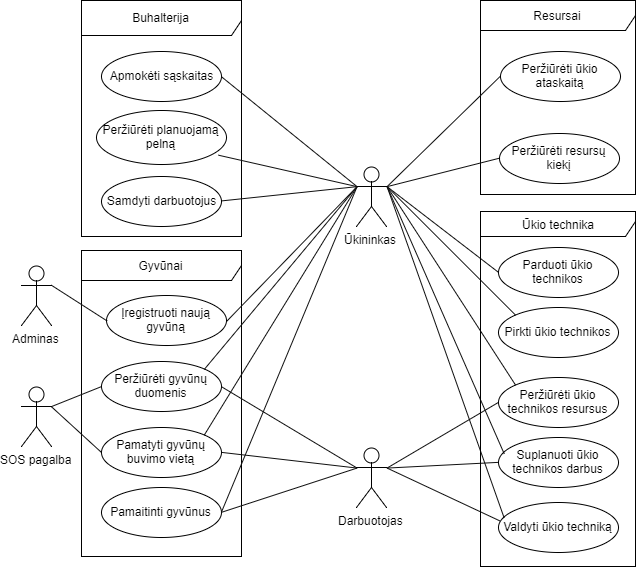
\includegraphics[width=15cm,height=17cm,keepaspectratio]{ResursaiUseCase.png}
	\caption{Use case. part 1}
	\label{fig:UseCaseFull}
\end{figure}
\item Šioje diagramoje pavaizduoti likusieji galimi veiksmai.
		\begin{figure}[H]
		\centering	
	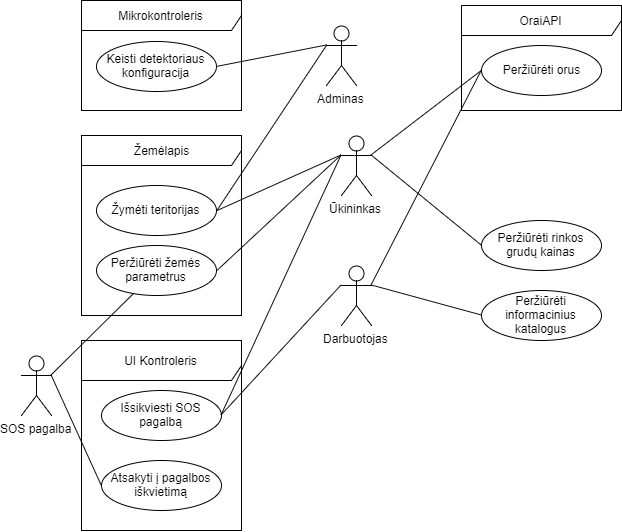
\includegraphics[width=15cm,height=17cm,keepaspectratio]{UseCase2.png}
	\caption{Use case. part 2}
	\label{fig:UseCaseFull}
\end{figure}
\end{itemize}

\subsection{Gyvūnų registracija}
	\subsubsection{Pagrindinis scenarijus}
	Vartotojas pasirenka ,,Gyvūnų registracija". Atsidariusiame lange vartotojas gali užregistruoti gyvūną. Vartotojui leidžiama pateikia tokius duomenis apie gyvūną: ID, lytis, svoris, amžius. Įvedęs duomenis vartotojas gali juos išsaugoti arba grįžti į pagrindinį programos langą.
	\subsubsection{Alternatyvus scenarijus(gyvūnas su tokiu ID jau egzistuoja)}
	Vartotojas pasirenka ,,Gyvūnų registracija". Atsidariusiame lange vartotojas bando įvesti ir išsaugoti gyvūno duomenis. Sistema patikrina, kad gyvūnas su tokiu ID jau egzistuoja. Vartotojui parodomas informacinis pranešimas dėl jau egzistuojančio gyvūno sistemoje ir paprašoma įvesti kitą ID arba grįžti į pagrindinį programos langą. 
	\subsubsection{Alternatyvus scenarijus(neteisingai įvesti duomenys)}
	Vartotojas pasirenka ,,Gyvūnų registracija". Atsidariusiame lange vartotojas bando įvesti ir išsaugoti gyvūno duomenis. Sistema patikrina įvestus duomenis ir pamato, kad vartotojas padarė formato klaidą įvesdamas duomenis. Vartotojui parodomas informacinis pranešimas kur buvo padaryta klaida ir paprašoma vartotojo pataisyti klaidingas vietas arba grįšti į pagrindinį meniu.
	\subsubsection{Funkciniai reikalavimai}

\begin{table}[htbp]
	\begin{tabularx}{1\textwidth}{ |P{2.5cm}|X|P{3cm }| }  \hline
	Nr. & Reikalavimas &  Prioritetas (1-10)  \\   \hline 
	FR-1.01 & Vartotojas gali užregistruoti gyvūną ir jo duomenis & 9  \\   \hline 
	FR-1.01.01 & Įvesti gyvūno ID & 9 \\   \hline
	FR-1.01.02 & Įvesti gyvūno lytį & 7 \\   \hline 
 	FR-1.01.03 & Įvesti gyvūno amžių & 7 \\   \hline
	FR-1.01.04 & Įvesti gyvūno svorį & 7 \\   \hline
	FR-1.02 & Parodyti informacinį pranešimą apie neteisingai įvestus duomenis & 8 \\   \hline
	
\end{tabularx}
\end{table}
\subsection{Gyvūnų lokacijos sekimas}
	\subsubsection{Pagrindinis scenarijus}
	Vartotojas pasirenka ,,Gyvūnų lokacijos sekimas". Sistema atidaro langą kuriame varotojui gali stebėti kiekvieno gyvūno lokaciją žemėlapyje . Vartotojui taip pat pateikiamas gyvūnų sąrašas kuriame galima pasirinkti vieną ar kelis gyvūnus stebėjimui. Saraše parašyta gyvūno ID ir tiksli gyvūno lokacija koordinatėmis. Vartotojui suteikiama galimybė grįžti į pagrindinį programos langą.
	\subsubsection{Alternatyvus scenarijus(Nėra gyvūnų kuriuos būtų galima stebėti)}
	Vartotojas pasirenka ,,Gyvūnų lokacijos sekimas" tačiau sistemoje nėra jokių užregistruotų gyvūnų. Vartotojui parodomas informacinis pranešimas apie įvykusia klaidą. Vartotojui suteikiama galimybė eiti į gyvūnų registracijos funkciją arba grįžti į pagrindinį meniu.
	\subsubsection{Alternatyvus scenarijus(Neveikia gyvūno lokacijos detektorius)}
	Vartotojas pasirenka ,,Gyvūnų lokacijos sekimas". Sistema parodo informacinį pranešimą, kad vienas arba kelis gyvūnų lokacijos detektoriai neveikia. Vartotojas informuojamas kurių gyvūnų(jų ID) detektoriai neveikia ir kokia buvo paskutinė gyvūnų lokaciją prieš detektoriui nustojant veikti.
	\subsubsection{Funkciniai reikalavimai}
\begin{table}[htbp]
	\begin{tabularx}{1\textwidth}{ |P{2.5cm}|X|P{3cm }| }  \hline
	Nr. & Reikalavimas &  Prioritetas (1-10)  \\   \hline 
	FR-3.01 & Vartotojui pateikiama kiekvieno gyvūno lokacija & 9 \\   \hline  
	FR-3.01.01 & Parodo gyvūną pagal pasirinktą ID & 7 \\   \hline 
	FR-3.01.02 & Leidžia pasirinkti kelis gyvūnus iš sąrąšo & 8 \\   \hline 
	FR-3.02 & Saugo gyvūno lokaciją sistemoje & 8 \\   \hline 
	FR-3.03 & Suteikia informaciją apie pabėgusius gyvūnus & 6 \\   \hline 

\end{tabularx}
\end{table}
	
\subsection{Gyvūnų duomenų peržiūra}
subsubsection{Pagrindinis scenarijus}
	Vartotojas pasirenka skiltį "Gyvūnų duomenų peržiūra", sistema atidaro sąrašą, kuriame išvardinti gyvūnai pagal id numerį, paspaudus ant id numerio iššoka langas, kuriame parodoma detalesnė gyvūno informacija. Norėdamas baigti vartotojas paspaudžia mygtuką ''Grįžti'', kuriuo nukreipiamas į pagrindinį meniu.
\subsubsection{Alternatyvus scenarijus(Nepavyksta pasiekti gyvūnų sąrašo)}
	Vartotojas pasirenka skiltį "Gyvūnų duomenų peržiūra", sistema išveda pranešimą, kad šiuo metu negali pasiekti gyvūnų duomenų, pasiūlo pabandyti vėliau, bet nukreipia atgal į pagrindinį meniu.
\subsubsection{Alternatyvus scenarijus(Sąrašas tuščias)}
	Vartotojas pasirenka skiltį "Gyvūnų duomenų peržiūra", sistema išveda pranešimą, kad gyvūnų sąrašas tuščias, bei pasiūlo pereiti į gyvūnų registraciją, vartotojui atsisakius grįžtama į pagrindinį meniu.
\subsubsection{Funkciniai reikalavimai}
\begin{table}[htbp]
	\begin{tabularx}{1\textwidth}{ |P{2.5cm}|X|P{3cm }| }  \hline
           	Nr. & Reikalavimas &  Prioritetas (1-10)  \\   \hline 
         	FR-3.01 & Sistema leidžia rikiuoti duomenis pagal: & 10  \\   \hline
		FR-3.01.01 & ID & 7 \\ \hline
		FR-3.01.02 & Svorį & 9 \\ \hline
		FR-3.01.02 & Amžių & 8 \\ \hline
        	FR-3.02 & Vartotojui pasirinkus gyvūno ID sistema parodo šiuos duomenis: & 10   \\   \hline
		FR-3.02.01 & ID & 9 \\ \hline
		FR-3.02.01 & Svorį & 9 \\ \hline
		FR-3.02.01 & Amžių & 9 \\ \hline
		FR-3.02.01 & Lytį & 8 \\ \hline
	\end{tabularx}
\end{table}

\subsection{Ūkio technikos resursų sekimas}
\subsubsection{Pagrindinis scenarijus}
	Vartotojas pasirenka skiltį "Ūkio technikos resursų sekimas", sistema parodo sąrašą, kuriame rodoma ūkio technika, jos užimtumas, būklė, darbo tvarkaraštis. duomenys pateikiami realiu laiku. Vartotojas pasirenka stebėti techniką realiu laiku, sistema parodo žemėlapį, kuriame matome, kur yra visos technikos priemonės, kiek apytiksliai laiko dirbs, ir ką darys toliau. Vartotojui baigus stebebėjimą grįžtama į pradinį meniu.
\subsubsection{Alternatyvus scenarijus(Nesukonfiguruoti priemonių sekikliai)}
	Vartotojas pasirenka skiltį "Technikos sekimas realiu laiku", sistema parodo sąrašą, kuriame rodoma ūkio technika, jos užimtumas, tačiau prie būklės rašoma klaida, jog nesukonfiguruotas priemonės sekiklis. Vartotojui sistema siūlo iškviesti sistemos administratorių, kuris sukonfiguruoja sekiklius ir nukreipia vartotoją į pagrindinį meniu.
\subsubsection{Alternatyvus scenarijus(Pasirinkta priemonė sugedus)}
	Vartotojas pasirenka skiltį "Technikos sekimas realiu laiku", sistema parodo sąrašą, kuriame rodoma ūkio technika, jos užimtumas, tačiau prie būklės rašoma klaida, jog priemonė sugedus. Sistema iškviečia mechaniką, išveda pranešimą, jog mechanikas iškviestas, ir nukreipia vartotoją į pagrindinį meniu.
\subsubsection{Funkciniai reikalavimai}
\begin{table}[htbp]
	\begin{tabularx}{1\textwidth}{ |P{2.5cm}|X|P{3cm }| }  \hline
           	Nr. & Reikalavimas &  Prioritetas (1-10)  \\   \hline 
         	FR-2.01 & Sistema leidžia vartotojui stebėti techniką & 10  \\   \hline
		FR-2.01.01 & Stebėti technikos būklę & 8 \\ \hline
		FR-2.01.02 & Peržiūrėti priemonės tvarkaraštį & 8 \\ \hline
		FR-2.01.03 & Stebėti priemonės veiklą realiu laiku & 8 \\ \hline
        	FR-2.02 & Sugedus priemonės sekikliui, programa leidžia iškviesti sistemos administratorių & 9   \\   \hline
		FR-2.03 & Sugedus priemonei, sistema iškviečia mechaniką & 9 \\ \hline
	\end{tabularx}
\end{table}

\subsection{Ūkio technikos resursų pirkimas}
\subsubsection{Pagrindinis scenarijus}
	Vartotojas pasirenka skiltį "Technikos sekimas realiu laiku", sistema parodo sąrašą, kuriame rodoma ūkio technika, jos užimtumas, būklė, darbo tvarkaraštis. Vartotojas pasirenka pirkti naują technikos priemonę, sistema nuveda jį į puslapį, kuriame yra pasiūlymai jo norimai technikos rūšiai pirkti. Vartotojui baigus grįžtama į pradinį meniu.
\subsubsection{Alternatyvus scenarijus(Nepavyko rasti skelbimų norimai priemonei)}
	Vartotojas pasirenka skiltį "Technikos sekimas realiu laiku", sistema parodo sąrašą, kuriame rodoma ūkio technika, jos užimtumas, būklė, darbo tvarkaraštis. Vartotojas pasirenka pirkti naują technikos priemonę, sistema nuveda jį į puslapį, kuriame yra pasiūlymai jo norimai technikos rūšiai pirkti, tačiau pasirinktai priemonei šiuo metu nėra sukurtų jokių skelbimų. Sistema išveda pranešimą, jog pasirinktos priemonės pasiūlymų nėra.
\subsubsection{Alternatyvus scenarijus(Nepavyko prisijungti prie serverio)}
	Vartotojas pasirenka skiltį "Technikos sekimas realiu laiku", sistema parodo sąrašą, kuriame rodoma ūkio technika, jos užimtumas, būklė, darbo tvarkaraštis. Vartotojas pasirenka pirkti naują technikos priemonę, tačiau sistemai nepavyko prisijungti prie serverio. Sistema išveda klaidos pranešimą ir nukreipia vartotoją į pagrindinį meniu.
\subsubsection{Funkciniai reikalavimai}
\begin{table}[htbp]
	\begin{tabularx}{1\textwidth}{ |P{2.5cm}|X|P{3cm }| }  \hline
           	Nr. & Reikalavimas &  Prioritetas (1-10)  \\   \hline 
         	FR-3.01 & Sistema leidžia vartotojui pirkti techniką & 10  \\   \hline
		FR-3.01.01 & Peržiūrėti skelbimus internete & 8 \\ \hline
        	FR-3.02 & Neradus norimos priemonės skelbimų, sistema išveda pranešimą & 8   \\   \hline
		FR-3.03 & Įvykus klaidai prisijungiant prie serverio, sistema išveda klaidos pranešimą ir nukreipia vartotoją į pagrindinį meniu & 8 \\ \hline
	\end{tabularx}
\end{table}

\subsection{Ūkio technikos resursų pardavimas}
\subsubsection{Pagrindinis scenarijus}
	Vartotojas pasirenka skiltį "Technikos sekimas realiu laiku", sistema parodo sąrašą, kuriame rodoma ūkio technika, jos užimtumas, būklė, darbo tvarkaraštis. Vartotojas pasirenka parduoti technikos priemonę, sistema patikrina, ar ši priemonė yra laisva, ir, jeigu ji nėra užimta, leidžia vartotojui sukurti skelbimą priemonei parduoti. sukūrus skelbimą grįžtama į pagrindinį meniu.
\subsubsection{Alternatyvus scenarijus(Priemonė, kurią norima parduoti, užimta)}
	Vartotojas pasirenka skiltį "Technikos sekimas realiu laiku", sistema parodo sąrašą, kuriame rodoma ūkio technika, jos užimtumas, būklė, darbo tvarkaraštis. Vartotojas pasirenka parduoti technikos priemonę, sistema patikrina, ar ši priemonė yra laisva, tačiau ji yra užimta. Sistema vartotojui leidžia pakeisti šios priemonės tvarkaraštį ir nustatyti, jog jo daugiau nebūtų galima pildyti. Sistema tuomet leidžia vartotojui sukurti skelbimą priemonei parduoti.
\subsubsection{Alternatyvus scenarijus(Priemonė, kurią norima parduoti, jau parduodama)}
	Vartotojas pasirenka skiltį "Technikos sekimas realiu laiku", sistema parodo sąrašą, kuriame rodoma ūkio technika, jos užimtumas, būklė, darbo tvarkaraštis. Vartotojas pasirenka parduoti technikos priemonę, sistema patikrina, ar ši priemonė yra laisva, tačiau jau yra sukurtas skelbimas jai parduoti. Vartotojui išvedamas klaidos pranešimas ir jis nuvedamas į ūkio technikos sąrašą.
\subsubsection{Funkciniai reikalavimai}
\begin{table}[htbp]
	\begin{tabularx}{1\textwidth}{ |P{2.5cm}|X|P{3cm }| }  \hline
    Nr. & Reikalavimas &  Prioritetas (1-10)  \\   \hline 
    FR-4.01 & Sistema leidžia vartotojui parduoti techniką & 10  \\   \hline
		FR-4.01.02 & Patikrinti, ar ši priemonė nėra jau parduodama & 8 \\ \hline
		FR-4.01.03 & Sukurti skelbimus internete & 9 \\ \hline
		FR-4.01.04 & Kuriant skelbimą sistema įveda ūkininko tel. numerį bei el. paštą į skelbimo informaciją & 8 \\ \hline
	\end{tabularx}
\end{table}

\subsection{Žemės parametrų sekimas}
\subsubsection{Pagrindinis scenarijus}
	Vartotojas pasirenka skiltį "Žemės parametrų sekimas", sistema nukreipia vartotoją į langą, kuriame yra sąrašas su visais prijungtais žemės parametrų sekikliais. Vartotojas pasirenka norimos teritorijos parametrų peržiūrą ir jam išvedami toje teritorijoje esančių daviklių duomenys. Vartotojui susipažinus su duomenimis grįžtamą į žemės parametrų detektorių sąrašą.
\subsubsection{Alternatyvus scenarijus(Nesukonfiguruotas daviklis)}
	Vartotojas pasirenka skiltį "Žemės parametrų sekimas", sistema nukreipia vartotoją į langą, kuriame yra sąrašas su visais prijungtais žemės parametrų sekikliais. Vartotojas pasirenka norimos teritorijos parametrų peržiūrą, tačiau toje teritorijoje nesukonfiguruotas daviklis. Sistema išveda pranešimą ir pasiūlo vartotojui iškviesti sistemos administratorių, kuris sukonfiguruotų neveikiantį daviklį, sistema vartotoją nukreipią į pagrindinį meniu.
\subsubsection{Alternatyvus scenarijus(Nepavyko prisijungti prie serverio)}
	Vartotojas pasirenka skiltį "Žemės parametrų sekimas", sistema nukreipia vartotoją į langą, kuriame yra klaidos pranešimas, jog nepavyko prisijungti prie serverio, ir vartotojas nukreipiamas atgal į pagrindinį meniu.
\subsubsection{Funkciniai reikalavimai}
\begin{table}[htbp]
	\begin{tabularx}{1\textwidth}{ |P{2.5cm}|X|P{3cm }| }  \hline
    Nr. & Reikalavimas &  Prioritetas (1-10)  \\   \hline 
    FR-5.01 & Sistema leidžia stebėti žemės parametrų sekiklių duomenis & 10  \\   \hline
		FR-5.02 & Atsiradus nesukonfiguruotam sekikliui, sistema leidžia iškviesti administratorių & 8 \\  \hline
		FR-5.03 & Nepavykus prisijungti prie serverio, vartotojas nukreipiamas į pagrindinį meniu & 8 \\ \hline
	\end{tabularx}
\end{table}

\subsection{Orų prognozės sekimas}
\subsubsection{Pagrindinis scenarijus}
	Vartotojas pasirenka skiltį "Orų prognozės sekimas", sistema vartotoją nukreipia į langą, kuriame jis gali pasirinkti artimiausią iki jo miestą ir peržiūrėti šios bei sekančios dienos orų prognozes.
\subsubsection{Alternatyvus scenarijus(Nėra prieigos prie interneto)}
	Vartotojas pasirenka skiltį "Orų prognozės sekimas", sistema vartotoją nukreipia į langą, kuriame jis gali pasirinkti artimiausią iki jo miestą, tačiau, pasirinkęs miestą, vartotojas gauna klaidos pranešimą, jog nepavyko prisijungti prie serverio, ir yra leidžiama varototojui bandyti pasirinkti miestą dar kartą prisijungus prie interneto.
\subsubsection{Alternatyvus scenarijus(Andromeda įsirėžė į Paukčių Tako galaktiką)}
	Vartotojas pasirenka skiltį "Orų prognozės sekimas", tačiau Andromeda įsirėžus į Paukščių Tako galaktiką ir nepavyksta gauti orų. Sistema išveda klaidos pranešimą ir nukreipia vartotoją į pagrindinį meniu.
\subsubsection{Funkciniai reikalavimai}
\begin{table}[htbp]
	\begin{tabularx}{1\textwidth}{ |P{2.5cm}|X|P{3cm }| }  \hline
      Nr. & Reikalavimas & Prioritetas (1-10)  \\   \hline 
      FR-6.01 & Sistema leidžia stebėti šios ir sekančios dienos orų prognozes & 10  \\   \hline
			FR-6.02 & Andromedai įsirėžus į Paukščių Tako galaktiką išvesti klaidos pranešimą & 1 \\  \hline
			FR-6.03 & Nepavykus prisijungti prie serverio, vartotojui leidžiama bandyti dar kartą prisijungus prie interneto & 7 \\ \hline
	\end{tabularx}
\end{table}

\subsection{Gyvūnų maitinimas}
\subsubsection{Pagrindinis scenarijus}
	Vartotojas pasirenka skiltį "Gyvūnų maitinimas", sistema atidaro langą, kuriame matoma kiek kokio maisto turima. Vartotojas gali pasirinkti maitinti gyvūnus, arba nustatyti laiką, kada automatiškai bus pamaitinti gyvūnai. Taip pat vartotojas gali pirkti maistą, sistema nukreipia varototoją į langą, kuriame jis gali pasirinkti kiek ir kokio maisto nori pirkti ir padaro užsakymą. Vartotojui suteikiama galimybė grįžti į pagrindinį programos.
\subsubsection{Alternatyvus scenarijus(Neužtenka maisto gyvūnų maitinimui)}
	Vartotojas pasirenka skiltį "Gyvūnų maitinimas", sistema atidaro langą, kuriame matoma kiek kokio maisto turima. Vartotojas pasirenka pamaitinti gyvunus, tačiau gauna klaidos pranešimą, jog sandelyje nėra pakankamai maisto norimam gyvūnų kiekiui pamaitinti. Vartotojas nukreipiamas į maisto pirkimo skiltį, kurioje jis gali sukurti maisto užsakymą.
\subsubsection{Alternatyvus scenarijus(Neužtenka maisto automatiniam gyvūnų maitinimui)}
	Vartotojas pasirenka skiltį "Gyvūnų maitinimas", sistema atidaro langą, kuriame matoma kiek kokio maisto turima. Vartotojas pasirenka pamaitinti gyvunus, tačiau gauna klaidos pranešimą, jog sandelyje nėra pakankamai maisto norimiem automatiniam maitinimam įgyvendinti. Vartotojas nukreipiamas į maisto pirkimo skiltį, kurioje jis gali sukurti maisto užsakymą.
\subsubsection{Funkciniai reikalavimai}
\begin{table}[htbp]
	\begin{tabularx}{1\textwidth}{ |P{2.5cm}|X|P{3cm }| }  \hline
    Nr. & Reikalavimas &  Prioritetas (1-10)  \\   \hline 
    FR-7.01 & Sistema leidžia maitinti gyvūnus & 10  \\   \hline
		FR-7.01.01 & Pamaitinti gyvūnus šiuo momentu & 8  \\ \hline
		FR-7.01.02 & Suplanuoti automatinius gyvūnų pamaitinimus & 8 \\ \hline
		FR-7.02 & Leidžia vartotojui sukurtu maisto užsakymus & 9 \\  \hline
	\end{tabularx}
\end{table}

\subsection{Ūkio technikos valdymas nuotolinių būdu realiu laiku}
\subsubsection{Pagrindinis scenarijus}
	Vartotojas pasirenka skiltį "Ūkio technikos valdymas", sistema atidaro langą, kuriame yra sąrašas ūkio technikos priemonių. Vartotojas pasirenka technikos priemonę ir, jei ji laisva, leidžia jos veikimą valdyti nuotoliniu būdu. Vartotojui baigus valdymą grįžtama į pagrindinį meniu.
\subsubsection{Alternatyvus scenarijus(Priemonė sugedus)}
	Vartotojas pasirenka skiltį "Ūkio technikos valdymas", sistema atidaro langą, kuriame yra sąrašas ūkio technikos priemonių. Vartotojas pasirenka technikos priemonę, tačiau ji yra sugedusi. Vartotojui pasiūloma iškviesti mechaniką priemonei sutvarkyti ir leidžia vartotojui pasirinkti kitą priemonę.
\subsubsection{Alternatyvus scenarijus(Priemonė užimta)}
	Vartotojas pasirenka skiltį "Ūkio technikos valdymas", sistema atidaro langą, kuriame yra sąrašas ūkio technikos priemonių. Vartotojas pasirenka technikos priemonę, tačiau gauna pranešimą, jog šią priemonę šiuo metu naudoja kažkas kitas. Vartotojui pasiūloma palaukti kol ji atsilaisvins arba pasirinkti kitą priemonę.
\subsubsection{Alternatyvus scenarijus(Nėra tinkamos įrangos)}
	Vartotojas pasirenka skiltį "Ūkio technikos valdymas", sistema atidaro langą, kuriame išvedamas klaidos pranešimas, jog nėra tinkamos įrangos priemonėm valdyti nuotoliniu būdu. Sistema pasiūlo vartotojui įsigyti šią įrangą ir nukreipia jį į pagrindinį meniu.
\subsubsection{Funkciniai reikalavimai}
\begin{table}[htbp]
	\begin{tabularx}{1\textwidth}{ |P{2.5cm}|X|P{3cm }| }  \hline
           	Nr. & Reikalavimas &  Prioritetas (1-10)  \\   \hline 
         		FR-8.01 & Sistema leidžia valdyti priemones nuotoliniu būdu & 10  \\   \hline
		FR-8.01.01 & Sistema patikrina, ar norima priemonė nėra užimta & 8  \\ \hline
		FR-8.01.02 & Sistema patikrina, ar norima priemonė nėra sugedusi & 7 \\ \hline
		FR-8.01.03 & Sistema patikrina, as yra tinkama įranga nuotoliniam valdymui & 7 \\  \hline
	\end{tabularx}
\end{table}

\subsection{Autonominis ūkio technikos veikimas}
\subsubsection{Pagrindinis scenarijus}
	Vartotojas pasirenka skiltį "Autonominis ūkio technikos veikimas", sistema atidaro langą, kuriame matomas technikos priemonių sąrašas. Vartotojas pasirenka priemonę, parenka plotą, kuriame priemonė dirbs, bei nustato norimą darbo laiką. Atlikus šiuos veiksmus sistema vartotoją nukreipia į pagrindinį meniu.
\subsubsection{Alternatyvus scenarijus(Priemonė užimta)}
	Vartotojas pasirenka skiltį "Autonominis ūkio technikos veikimas", sistema atidaro langą, kuriame matomas technikos priemonių sąrašas. Vartotojas pasirenka priemonę, tačiau ji šiuo metu jau dirba. Vartotojui pasiūloma suplanuoti automatinį darbą kai priemonė atsilaisvins arba pasirinkti kitą priemonę.
\subsubsection{Alternatyvus scenarijus(Priemonė neturi tinkamos įrangos)}
	Vartotojas pasirenka skiltį "Autonominis ūkio technikos veikimas", sistema atidaro langą, kuriame matomas technikos priemonių sąrašas. Vartotojas pasirenka priemonę, tačiau ji neturi tinkamos įrangos autonominiam veikimui. Sistema išveda pranešimą pasiūlo įsigyti įrangą arba pasirinkti kitą priemonę.
\subsubsection{Alternatyvus scenarijus(Netinkamas pasirinktas plotas)}
	Vartotojas pasirenka skiltį "Autonominis ūkio technikos veikimas", sistema atidaro langą, kuriame matomas technikos priemonių sąrašas. Vartotojas pasirenka priemonę ir parenka plotą, kuriame priemonė dirbs, tačiau tame plote yra ne ariamas laukas. Sistema išveda klaidos pranešimą ir prašo vartotojo patikslinti darbo plotą.
\subsubsection{Funkciniai reikalavimai}
\begin{table}[htbp]
	\begin{tabularx}{1\textwidth}{ |P{2.5cm}|X|P{3cm }| }  \hline
    Nr. & Reikalavimas &  Prioritetas (1-10)  \\   \hline 
    FR-9.01 & Sistema leidžia suplanuoti autonominį technikos priemonės darbą & 10  \\   \hline
		FR-9.01.01 & Sistema patikrina, ar norima priemonė nėra užimta & 8  \\ \hline
		FR-9.01.02 & Sistema patikrina, ar norima priemonė nėra sugedusi & 7 \\ \hline
		FR-9.01.03 & Sistema patikrina, ar yra tinkama įrangą autonominiam veikimui & 7 \\  \hline
		FR-9.01.04 & Sistema patikrina, ar tinkamai pažymėtas darbo plotas & 9  \\ \hline
	FR-9.01.04.01 & Ar pažymėtas laukas tinkamas pasirinktai ūkio technikos priemonei jame dirbti & 8 \\ \hline
	\end{tabularx}
\end{table}

\subsection{Ūkininko valdomos teritorijos žymėjimas sutartiniais ženklais}
	\subsubsection{Pagrindinis scenarijus}
	Vartotojas pasirenka ''Žemėlapio žymėjimas'' pagrindiniame meniu. Programa atidaro langą, kuriama vartotojas pasirenka norimą plotą pasirinktoje vietoje. Atlikus žimėjimą sistema pasiūlo pažymeti dar vieną plotą, vartotojui atsisakius grįžtama į pagrindinį meniu.
	\subsubsection{Alternatyvus scenarijus(Plotas priklauso kitam savininkui)}
	Vartotojas pasirenka ''Žemėlapio žymėjimas'' pagrindiniame meniu. Programa atidaro langą, kuriama vartotojas pasirenka norimą plotą pasirinktoje vietoje, tačiau tas plotas priklauso kitam ūkininkui. Sistema išveda pranešimą, kad ši teritoja ūkininkui nepriklauso, bei atšaukia esamą žymėjimą.
	\subsubsection{Alternatyvus scenarijus(Plotas jau pažymėtas)}
	Vartotojas pasirenka ''Žemėlapio žymėjimas'' pagrindiniame meniu. Programa atidaro langą, kuriama vartotojas pasirenka norimą plotą pasirinktoje vietoje, tačiau tas plotas jau pažymėtas. Sistema išveda pranešimą, bei pasiūlo pakeisti ploto paskirtį.
	\subsubsection{Funkciniai reikalavimai}
	\begin{table}[htbp]
		\begin{tabularx}{1\textwidth}{ |P{2.5cm}|X|P{3cm }| }  \hline
			Nr. & Reikalavimas & Prioritetas(1-10) \\ \hline
			FR-12.01 & Sistema leidžia pasirinkti žymimo ploto paskirtį & 10 \\ \hline
			FR-12.01.01 & Ariamas laukas & 10 \\ \hline
			FR-12.01.02 & Ūkinis pastatas & 10 \\ \hline
			FR-12.01.03 & Ganykla & 10 \\ \hline
			FR-12.02 & Sistema leidžia ištrinti jau pasirinką plotą & 9 \\ \hline
			FR-12.03 & Sistema leidžia pakeisti jau pažymeto ploto paskirtį & 9 \\ \hline
			FR-12.04 & Paspaudus ant pažymeto ploto sistema išveda to ploto informaciją & 10 \\ \hline
			FR-12.04.01 & Paskirtį & 10 \\ \hline
			FR-12.04.02 & Plotą & 10 \\ \hline			
		\end{tabularx}
	\end{table}
\subsection{Sąskaitų išrašymas}
	\subsubsection{Pagrindinis scenarijus}
	Vartotojas pasirenka skiltį "Sąskaitos". Atsidariusiame lange vartotojui parodo sąrašą visų sąskaitų, kurias jam reikia apmokėti. Šalia kiekvienos sąskaitos yra mygtukas, kurį paspaudus vartotojas nukreipiamas į apmokėjimo platformą pagal vartotojo pasirinkimą, kurioje jis gali apmokėti konkrečią sąskaitą. Pagrindiniame sąskaitų lange vartotojas gali pasižiūrėti, kokia sąskaitos suma, ir kada ji buvo išrašyta. Taip pat gali pasižiūrėti jau apmokėtų sąskaitų istoriją. Apmokėjus sąskaitą vartotojas nukreipiamas į dar neapmokėtų sąskaitų sąrašą, jeigu jau visos sąskaitos apmokėtos parodomas apmokėtų sąskaitų sąrašas.
	\subsubsection{Alternatyvus scenarijus(Nėra sąskaitų, kurias reiktų apmokėti)}
	Jeigu sistemoje nėra sąskaitų, kurias vartotojas turėtų apmokėti, vartotojui paspaudus ant "Sąskaitos" mygtuko jam bus parodytas informacinis langas, pranešantis, kad nėra sąskaitų, kurias šiuo metu reiktų apmoketi. Lange bus galima pasirinkti arba eitį į pagrindinį meniu, arba peržiūrėti sąskaitų istoriją.
	\subsubsection{Alternatyvus scenarijus(Nėra jau apmokėtų sąskaitų)}
	Jeigu vartotojas "Sąskaitos" lange bandys peržiūrėti sąskaitų istoriją ir joje nieko nebus, vartotojui bus parodomas informacinis langas, kuriame bus pranešimas "Sąskaitų istorijos nėra", ir vartotojas bus nukreipiamas į sąskaitas, kurias reikia apmokėti, arba į alternatyvų scenarijų, kai nėra sąskaitų, kurias reiktų apmokėti.
	\subsubsection{Alternatyvus scenarijus(Negalima pasiekti pasirinktos apmokėjimo sistemos)}
	Vartotojui bandant apmokėti savo sąskaitas jis gali pasirinkti iš keletos apmokėjimo platformų. Jeigu jo pasirinkta apmokėjimo platforma atmeta vartotojo apmokėjimo prašymą dėl nepakankamų lėšų, neveikiančios apmokėjimo sistemos ar kitų nenumatytų nesklandumų, sistema parodys informacini pranešimą "Sąskaitos apmokėti nepavyko". Po pranešimu sistema parodys alternatyvius apmokėjimo būdus, o jeigų tokių būdų nėra, sistema parodys apmokėjimo informaciją, su kuria vartotojas sąskaitą galės apmokėti pats, neautomatiškai.
	\subsubsection{Funkciniai reikalavimai}
\begin{table}[htbp]
	\begin{tabularx}{1\textwidth}{ |P{2.5cm}|X|P{3cm }| }  \hline
		Nr. & Reikalavimas & Prioritetas(1-10) \\ \hline
		FR-14.01 & Sistema leidžia peržiūrėti sąskaitas & 10 \\ \hline
		FR-14.01.01& Peržiūrėti sąskaitas, kurias reikia apmokėti & 10 \\ \hline
		FR-14.01.02 & Peržiūrėti apmokėtų sąskaitų istoriją & 7 \\ \hline 
		FR-14.01.03 & Laikyti sąskaitų istoriją ilgiau negu pusę metų & 5 \\ \hline
		FR-14.02 & Amokėti sąskaitą & 7 \\ \hline
		FR-14.02.01 & Pateikti apmokėjimo platformų sąrašą & 9 \\ \hline
		FR-14.02.02 & Suteikti apmokėjimo informaciją & 10 \\ \hline
	\end{tabularx}
\end{table}
\subsection{Darbuotojų samdymas}
	\subsubsection{Pagrindinis scenarijus}
	Vartotojas pasirenka skiltį "Darbuotojų samdymas". Vartotojui parodomas langas su dviem pasirinkimais: "Dėti darbo skelbimą" ir "Žiūrėti darbo skelbimus". Pasirinkus pirmąjį pasirinkimą, vartotojas nukreipiamas į formą, kurią vartotojas turi užpildyti apie norimą darbuotoją. Paspaudus antrajį pasirinkimą, vartotojas nukreipiamas į darbo skelbimus, kurie jau yra internete.
	\subsubsection{Alternatyvus scenarijus(Neatsidaro darbo skelbimų puslapis)}
	Vartotojas bando atidaryti darbo skelbimų puslapį, spausdamas "Žiūrėti darbo skelbimus". Nepavykus pateikti puslapio vartotojui, ekrane atsiranda informacinis pranešimas, kad darbo skelbimų parodyti nepavyko, ir vartotojas bus perkeliamas į pagrindinį programos puslapį.
	\subsubsection{Alternatyvus scenarijus(Neteisingai suvesti duomenys bandant įdėti darbo skelbimą)}
	Vartotojas bando užpildyti formą ir įdėti skelbimą, bet padaro įvedimo klaidą(pvz. į siūlomos algos vietą įveda raides). Programa pažymi vietą, kur vartotojas padarė klaidą, ir neleidžia išsiųsti skelbimo kol formoje yra klaidų.
	\subsubsection{Funkciniai reikalavimai}
\begin{table}[htbp]
	\begin{tabularx}{1\textwidth}{ |P{2.5cm}|X|P{3cm }| }  \hline
		Nr. & Reikalavimas & Prioritetas(1-10) \\ \hline
		FR-15.01 & Sistema leidžia peržiūrėti darbo skelbimų sąrašą & 9 \\ \hline
		FR-15.01.01 & Surūšiuoti darbuotojus pagal lytį & 7 \\ \hline
		FR-15.01.02 & Surūšiuoti darbuotojus pagal amžių & 7 \\ \hline
		FR-15.01.03 & Surūšiuoti darbuotojus pagal specialybę & 8  \\ \hline
		FR-15.01.04 & Surūšiuoti darbuotojus pagal darbo patirtį & 8 \\ \hline
		FR-15.01.05 & Surūšiuoti darbuotojus pagal gyvenamąją vietą & 7 \\ \hline
		FR-15.01.06 & Peržiūrėti darbuotojų gyvenimo aprašymus & 9 \\ \hline
		FR-15.01.07 & Peržiūrėti darbuotojų motyvacinius laiškus & 5 \\ \hline
		FR-15.02 & Sistema leidžia užpildyti darbo skelbimą & 9 \\ \hline
		FR-15.02.01 & Pasirinkti vieną ar kelias skelbimų publikavimo platformamas & 8 \\ \hline
		FR-15.02.02 & Ištrinti darbo skelbimą & 9 \\ \hline
		FR-15.02.03 & Koreguoti darbo skelbimą & 8 \\ \hline
	\end{tabularx}
\end{table}	

\subsection{Potencialaus pelno skaičiavimas}
	\subsubsection{Pagrindinis scenarijus}
	Vartotojas pasirenka "Potencialaus pelno skaičiavimas" sistemoje. Programa įjungia langą, kuriame yra sąrašas visų šiuo metu vartotojo turimų pardavimui skirtų resursų. Vartotojas gali pasirinkti žiūrėti bendrą pelną, kurį gautų pardavęs resursus, arba pasirinkti tam tikrus resursus, kuriuos norėtų parduoti, ir kokį kiekį norėtų parduoti. Pagal vartotojo pasirinkimą ir rinkos kainą yra apskaičiuojamas potencialus pelnas. Vartotojui susipažinus su potencialiu pelnu grįžtama į pagrindinį meniu.
	\subsubsection{Alternatyvus scenarijus(Nartotojas neturi parduodamų resursų)}
	Vartotojas pasirenka "Potencialaus pelno skaičiavimas" skiltį. Sistemoje nėra užregistruota jokių resursų, kuriuos vartotojas galėtų parduoti. Vartotojui parodomas pranešimas apie nepavykusią operaciją dėl resursų trūkumo. Programa įjungia pagrindinį langą. 
	\subsection{Alternatyvus scenarijus(Neveikia išoriniai servisai, suteikiantys informaciją apie rinkos kainas)}
	Vartotojas pasirenka "Potencialaus pelno skaičiavimas" skiltį. Norint apskaičiuoti potencialų pelną naudojamas išorinis servisas nustatyti rinkos kainą. Šiam servisui neveikiant programa vartotojui parodo informacinį pranešimą dėl nesėkmingo bandymo susisiekti su išoriniu servisu. Tokiu atveju programa naudoja naujausią turėtą rinkos kainą pelno skaičiavimui. Dėl senų duomenų naudojimo ir galimų netikslumų vartotojas taip pat informajamas informacine žinute.
	\subsubsection{Funkciniai reikalavimai}
\begin{table}[htbp]
	\begin{tabularx}{1\textwidth}{ |P{2.5cm}|X|P{3cm }| }  \hline
		Nr. & Reikalavimas & Prioritetas(1-10) \\ \hline
		FR-16.01 & Sistema pateikia vartotojui potencialų pelną & 10 \\ \hline
		FR-16.01.01 & Pasirinkti, kuriuos resursus skaičiuoti & 8 \\ \hline
		FR-16.01.02 & Pasirinkti resursų kiekį skaičiavimui & 8 \\ \hline
		FR-16.01.03 & Pasirinkti, pagal kuriuos rinkos duomenis skaičiuoti pelną & 8 \\ \hline
	\end{tabularx}
\end{table}	
\subsection{Derliaus sekimas}
	\subsubsection{Pagrindinis scenarijus}
	Vartotojas sistemoje pasirenka "Derliaus sekimas". Programa įjungią vartotojo turimų resursų sąrašą. Saraše prie kiekvieno resurso parašyta, kada jis buvo gautas ir kokia kiekvieno resurso galiojimo trukmė. Paspaudus ant konkretaus resurso pasirodo langas, kuriame pateikta detalesnė informacija apie konkretų resursą. Detali informacija susideda iš resurso gavimo laiko, darbuotojų kurie dirbo prie konkretaus resurso gavimo, kiek pinigų vartotojas gautų pardavęs resursus rinkos kaina. Vartotojui baigus peržiūrą grįžtama į pagrindinį meniu.
	\subsubsection{Alternatyvus scenarijus(Vartotojas neturi resursų, kuriuos būtų galima parodyti)}
	Vartotojas sistemoje pasirenka "Derliaus sekimas". Sistemoje nėra užregistruota jokių resursų. Vartotojui parodomas informacinis pranešimas apie tai, kad sistemoje nėra registruotų resursų. Vartotojas nukreipiamas į pagrindinį langą.
	\subsubsection{Alternatyvus scenarijus(Neveikia rinkos skaičiavimo funkcija)}
	Vartotojas sistemoje pasirenka "Derliaus sekimas". Sistema atidaro langą su resursais. Vartotojas pasirenka konkretų resursą, norėdamas sužinoti detalesnią informaciją. Rinkos kainos funkcija dėl tam tikrų priežasčių neveikia ir neįmanoma parodyti tikslios rinkos kainos. Vartotojui parodomas informacinis pranešimas dėl netikslios kainos. Taip pat vartotojas informuojamas, kad preliminari kaina bus skaičiuojama naudojantis senais rinkos duomenimis.
	\subsubsection{Funkciniai reikalavimai}
\begin{table}[htbp]
	\begin{tabularx}{1\textwidth}{ |P{2.5cm}|X|P{3cm }| }  \hline
		Nr. & Reikalavimas & Prioritetas(1-10) \\ \hline
		FR-17.01 & Sistema vartotojui pateikia turimų resursų sąrašą & 10 \\ \hline
		FR-17.01.01 & Pateikti turimų resursų kiekį & 8 \\ \hline
		FR-17.01.02 & Pateikti turimų resursų galiojimo laiką & 8 \\ \hline
		FR-17.01.03 & Pateikti laiką, kada buvo gautas konkretus resursas & 8 \\ \hline
		FR-17.01.04 & Pateikti sąrašą žmonių, kurie dirbo prie konkretaus resurso gavimo & 6 \\ \hline
		FR-17.01.05 & Pateikti resurso rinkos kainą & 7 \\ \hline 
		FR-17.01.06 & Pateikti, kiek pinigų vartotojas gautų pardavęs konkretų resursą pagal rinkos kainą & 7 \\ \hline
	\end{tabularx}
\end{table}	
	
\subsection{Buhalterijos tvarkymas}
	\subsubsection{Pagrindinis scenarijus}
	Vartotojas pasirenka "Buhalterijos tvarkymas" pagrindiniame meniu. Programa atidaro langą, kuriame vartotojas nukreipiamas į buhalterijos tvarkymo platformą. Vartotojas prisijungia prie platformos naudodamas savo duomenis.
	\subsubsection{Alternatyvus scenarijus(Neveikia buhalterijos servisas)}
	Vartotojas pasirenka "Buhalterijos tvarkymas". Išorinis buhalterijos servisas neveikia. Vartotojui parodomas informacinis pranešimas, kad dėl tam tikrų priežasčių buhalterijos tvarkymo servisas šiuo metu neveikia. Vartotojas nureipiamas į darbalaukio aplikaciją, kurioje ji gali tvarkyti buhalteriją.
	\subsubsection{Funkciniai reikalavimai}
	\begin{table}[htbp]
	\begin{tabularx}{1\textwidth}{ |P{2.5cm}|X|P{3cm }| }  \hline
		Nr. & Reikalavimas & Prioritetas(1-10) \\ \hline
		FR-18.01 & Sistema suteikia vartotojui prieigą prie buhalterijos tvarkymo platformos & 9 \\ \hline
	\end{tabularx}
\end{table}
\subsection{Rinkos kainų sekimas}
	\subsubsection{Pagrindinis scenarijus}
	Vartotojas pagrindiniame lange pasirenka "Rinkos kainų sekimas". Programa atidaro langą, kuriame rodomos resursų kainos realiu laiku. Vartotojas gali pasirinkti laiko intervalą, kuriame nori stebėti rinkos kainos pokyčius, ir kurių resursų kainas stebėti. Vartotojas taip pat gali grįžti į pagrindinį programos langą.
	\subsubsection{Atlernatyvus scenarijus(Nepavyksta gauti rinkos kainų)}
	Vartotojas pagrindiniame lange pasirenka "Rinkos kainų sekimas". Dėl tam tikrų priežasčių nepavyksta gauti dabartinės rinkos kainos. Vartotojui parodomas informacinis pranešimas dėl netikslių rinkos duomenų. Vartotojui parodoma rinkos kainų istorija, kuri yra saugoma sistemoje. Taip pat suteikiama galimybė sugrįši į pagrindinį sistemos langą.
	\subsubsection{Alternatyvus scenarijus(Nepavyksta gauti rinkos kainų istorijos)}
	Vartotojas pagrindiniame lange pasirenka "Rinkos kainų sekimas". Dėl nenumatytų nesklandumų nepavyksta gauti dabartinių rinkos kainų ir sistemoje nėra išsaugota kainų istorija. Vartotojas informuojamas, kad nepavyksta gauti rinkos kainų realiu laiku, ir kad sistemoje nėra išsaugotos kainų istorijos. Vartotojas nukreipiamas į pagrindinį programos langą.
	\subsubsection{Funkciniai reikalavimai}
\begin{table}[htbp]
	\begin{tabularx}{1\textwidth}{ |P{2.5cm}|X|P{3cm }| } \hline
		Nr. & Reikalavimas & Prioritetas(1-10) \\ \hline
		FR-19.01 & Sistema parodo rinkos kainas realiu laiku &  9 \\ \hline
		FR-19.01.01 & Leisti pasirinkti konkrečius resursus jų kainos rodymui & 8 \\ \hline
		FR-19.01.02 & Rodyti rinkos kainų istoriją & 7 \\ \hline
		FR-19.01.03 & Saugoti rinkos kainų istoriją & 7 \\ \hline
	
	\end{tabularx}
\end{table}
	 
\subsection{Automatinis žemės laistymas}
	\subsubsection{Pagrindinis scenarijus}
	Vartotojas pagrindiniame programos lange pasirenka "Automatinis žemė laistymas". Programa atidaro automatinės laistymo sistemos langą. Lange vartotojui yra pateikiama informacija kokia žemės dregmė kiekviename žemės plote. Vartotojas gali pasirinkti kokiai žemės drėgmei esant sistema automatatiškai įjungtų žemės laistytuvus. Vartotojui pateikiama informacija apie laistytuvų būklę(veikia, neveikia). Sistema suteikia galimybę pasirinkti kokiu laiku sistema palaistys žemę. Taip pat yra suteikiama galimybė žemę palaistyti dabar. Atlikus norimus veiksmus vartotojui suteikiama galimybė grįžti į pagrindinį programos langą.
	\subsubsection{Alternatyvus scenarijus(Nepavyksta nusiųsti informacijos laistymo sistemai)}
	Vartotojas pasirenka "Automatinis žemės laistymas". Programa atidaro laistymo sistemos langą. Vartotojas bando pakeisti laistymo nustatymus tačiau nepavyksta nurodymų nusiųsti valdikliams. Vartotojas informuojamas informacine žinute, kad naujų nustatymų nusiųsti nepavyko ir sistema toliau dirbs pagal senus nustatymus. Vartotojui suteikiami keli pasirinkimai: atlikti sistemos diagnostika, išjungti sistemą rankiniu būdu(kartu su instrukcijomis kaip tai padaryti), iškviesti sistemos techniką arba grįžti į pagrindinį programos langą.
	\subsubsection{Alternatyvus scenarijus(Sisemoje nėra vandens)}
	Vartotojas pasirenka "Automatinis žemės laistymas". Vartotojui parodomas informacinis pranešimas dėl vandens tiekimo sutrikimo sistemoje. Vartojui siūloma atlikti diagnostika arba papildyti vandens talpas rankiniu būdu(parodomas instrukcinis pranešimas kaip tai padaryti) arba vartotojas gali grįšti į pagrindinį programos meniu.
	\subsubsection{Alternatyvus scenarijus(Neatsidaro vandens vožtuvai laistymui)}
	Vartotojas pasirenka "Automatinis žemės laistymas". Vartotojas informuojamas, kad dėl sistemos gedimo nepavyksta atidaryti vandens vožtuvų. Vartotojas informuojamas, kad įvyko gedimas ir reikia gedimą pašalinti prieš tęsiant darbą. Vartotojui suteikiama galimybė išsikviesti sistemos techniką arba susitvarkyti pačiam(pateikiama instrukcija kaip tai padaryti).  Vartotojas taip pat gali grįšti į pagrindinį programos langą.
	\subsubsection{Funkciniai reikalavimai}
\begin{table}[htbp]
	\begin{tabularx}{1\textwidth}{ |P{2.5cm}|X|P{3cm }| } \hline
		Nr. & Reikalavimas & Prioritetas(1-10) \\ \hline
		FR-20.01 & Sistema leidžia vartotojui matyti laukus ir kontroliuoti laistymo sistemą & 9 \\ \hline
		FR-20.01.01 & Laistyti dabar & 7 \\ \hline
		FR-20.01.02 & Nustatyti laistymo laiko & 8\\ \hline
		FR-20.01.03 & Nustatyti kokiai drėgmei esant laistyt žemę & 8 \\ \hline
		FR-20.01.04 & Suteikti informaciją apie žemės dregmę & 7 \\ \hline
		FR-20.01.05 & Suteikti informaciją apie laistytuvų būklę & 7 \\ \hline
		FR-20.01.06 & Suteikti diagnostikos galimybes neveikimo atveju & 8 \\ \hline
		FR-20.01.07 & Suteikti informaciją apie sistemos pataisymo galimybes & 8 \\ \hline
	\end{tabularx}
\end{table}
\subsection{Pagalbos iškvietimas}
	\subsubsection{Pagrindinis scenarijus}
	Vartotojas pasirenka ''Pagalbos iškvietimas'' pagrindiniame meniu. Programa atidaro langą, kuriama vartotojas pasirenka reikiamos pagalbos tipą, sistema tada nusiunčia skubų numatytąjį pranešimą su prašymų atvykti, vartotojui praneša, kad pranešimas išsiųstas, bei praneša, kai gavėjas jį pamato. Vartotojui suteikiama galimybė išsiūsti kitą pagalbos pranešimą arba grįšti į pagrindinį langą.
	\subsubsection{Alternatyvus scenarijus(nėra interneto ryšio)}
	Vartotojas pasirenka ''Pagalbos iškvietimas'' pagrindiniame meniu. Programa atidaro langą, kuriama vartotojas pasirenka reikiamos pagalbos tipą, sistemai nepavykus išsiųsti pranešimo parodomas pranešimas, kuriame nurodoma, kokiu numeriu reikia paskambinti norint išsikviesti norimą pagalbą. Vartotojui suteikiama galimybė grįžti į pagrindinį langą.
	\subsubsection{Funkciniai reikalavimai}
	\begin{table}[htbp]
		\begin{tabularx}{1\textwidth}{ |P{2.5cm}|X|P{3cm }| }  \hline
			Nr. & Reikalavimas & Prioritetas(1-10) \\ \hline
			FR-21.01 & Sistema leidžia pasirinkti reikiamos pagalbos tipą & 10 \\ \hline
			FR-21.01.01 & Veterinarą & 9 \\ \hline
			FR-21.01.02 & Agronomą & 8 \\ \hline
			FR-21-02 & Vartotojui pasirinkus sistema iškviečia pasirinktą pagalbą & 10 \\ \hline	
			FR-21-02.01 & Parodo gautą atsakymą iš pagalbos suteikėjo & 9 \\ \hline
			FR-21-03 & Sistema leidžia nustatyti numatytąjį pranešimą, siunčiamą kiekvienai pagalbai & 9 \\ \hline	
			FR-21-03 & Nesant galimybės nusiųsti pranešimui sistema parodo atitinkamos pagalbos kontaktus & 10 \\ \hline	
			FR-21-03.01 & Tel. numerį & 10 \\ \hline	
			FR-21-03.02 & Adresą & 8 \\ \hline	
			FR-21-03.03 & El. paštą & 6 \\ \hline						
		\end{tabularx}
	\end{table}
\subsection{Ataskaitos apie ūkį sudarymas}
	\subsubsection{Pagrindinis scenarijus}
	Vartotojas pasirenka ''Ūkio ataskaita'' pagrindiniame meniu. Programa atidaro langą, kuriame vartotojas pasirenka norimą laikotarpį, ir peržiūri to laikotarpio ataskaitą. Peržiūrėjęs ataskaita vartotojas gali baigti darbą ir grįžti į pagrindinį langą arba vėl vesti laikotarpį ir gauti naują ataskaitą.
	\subsubsection{Alternatyvus scenarijus(Nepasiekiama duomenų bazė)}
	Vartotojas pasirenka ''Ūkio ataskaita'' pagrindiniame meniu. Programa atidaro langą, kuriame vartotojas pasirenka norimą laikotarpį. Programa išveda klaidos pranešimą ir pasiūlo pamėginti vėliau ir suteikiama galimybė grįžti į pagrindinį programos langą.
	\subsubsection{Funkciniai reikalavimai}
	\begin{table}[htbp]
		\begin{tabularx}{1\textwidth}{ |P{2.5cm}|X|P{3cm }| }  \hline
			Nr. & Reikalavimas & Prioritetas(1-10) \\ \hline
			FR-22.01 & Sistema leidžia pasirinkti norimą laikotarpį ataskaitai & 9 \\ \hline
			FR-22-02 & Sistema sudaro ataskaitą vartotojo pasirinktam laikotarpiui & 10 \\ \hline	
		\end{tabularx}
	\end{table}
\subsection{Žolių, ligų ir ūkio chemijos katalogas}
	\subsubsection{Pagrindinis scenarijus}
	Vartotojas pasirenka ''Žolių ir ligų katalogas'' pagrindiniame meniu. Programa atidaro langą, kuriame vartotojas gali matyti pasirinktą katalogą, jame ieškoti ir peržiūrėti konkrečia ligą arba žolę. Pabaigęs darbą vartotojas turi galimybę grįšti į pagrindinį meniu.
	\subsubsection{Alternatyvus scenarijus(Nesėkminga paieška)}
	Vartotojas pasirenka ''Žolių ir ligų katalogas'' pagrindiniame meniu. Programa atidaro langą, kuriame rodomas katalogas. Vartotojui atlikus paiešką ir neradus jokių rezultatų išvedamas pranešimas, kad tokių duomenų kataloge nėra. Vėl parodomas pilnas katalogas ir vartotojas gali daryti kitą paieškos užklausą.
	\subsubsection{Funkciniai reikalavimai}
	\begin{table}[htbp]
		\begin{tabularx}{1\textwidth}{ |P{2.5cm}|X|P{3cm }| }  \hline
			Nr. & Reikalavimas & Prioritetas(1-10) \\ \hline
			FR-24.01 & Sistema leidžia pasirinkti norimą katalogą & 10 \\ \hline
			FR-24.01.01 & Žolelių & 10 \\ \hline
			FR-24.01.02 & Ūkio chemijos & 10 \\ \hline
			FR-24.01.03 & Gyvūnų ligų & 9 \\ \hline
			FR-24.01.04 & Žmonių ligų & 7 \\ \hline
			FR-24.01.02 & Pasirinkus katalogo elementą sistema pateikia informaciją apie jį & 9 \\ \hline
			FR-24.03 & Sistema leidžia atlikti paiešką  & 9 \\ \hline
			FR-24.03.01 & Pagal simbolių eilutę esančią pavadinime & 9 \\ \hline
			FR-24.03.01 & Pagal simbolių eilutę esančią aprašyme & 8 \\ \hline
			FR-24.04 & Sistema leidžia norimą katalogą rikiuoti & 9 \\ \hline
			FR-24.04.01 & Pagal alfabetinę tvarką  & 9 \\ \hline
		\end{tabularx}
	\end{table}
	
	\subsection{Atsakymas į pagalbos iškvietimą}
	\subsubsection{Pagrindinis scenarijus}
	Pagalbos teikėjas pasirenka skiltį ''pagalbos prašymai'' pasirenką norimą pagalbos prašymą ir parašo pranešimą siuntėjui su informacija kada atvyks, kiekvienas pagalbos prašymas pradingta po 24h.
	\subsubsection{Alternatyvus scenarijus(Nėra pagalbos prašymų)}
	Pagalbos teikėjas pasirenka skiltį ''pagalbos prašymai'', jam sistema parodo pranešimą, kad šiuo metu jokių pagalbos prašymų nėra, jis grąžinamas į pagrindinį langą.
	\subsubsection{Funkciniai reikalavimai}
	\begin{table}[htbp]
		\begin{tabularx}{1\textwidth}{ |P{2.5cm}|X|P{3cm }| }  \hline
			Nr. & Reikalavimas & Prioritetas(1-10) \\ \hline
			FR-24.01 & Sistema turi leisti išsiųsti atsakymą pagalbos iškvietėjui & 10 \\ \hline
			FR-24.02 & Prieš išsiunčiant atsakymą, pagalbos teikėjas turi įvesti planuojamą atvykimo laiką & 9 \\ \hline
		\end{tabularx}
	\end{table}
	
	\subsection{Detektoriaus konfiguracijos keitimas}
	\subsubsection{Pagrindinis scenarijus}
	Administratorius pasirenką ''Detektorių kodavimas'' pagrindiniame meniu, naujame lange pasirenka norimą koduotį detektorių. Po šio veiksmo iššoka langas, kuriame Administratorius gali keisti detektoriaus konfiguraciją, jam paspaudus mygtuką ''išsaugoti'' grįžtama į pagrindinį meniu.
	\subsubsection{Alternatyvus scenarijus(Negalima pasiekti detektoriaus)}
	Administratorius pasirenką ''Detektorių kodavimas'' pagrindiniame meniu, naujame lange pasirenka norimą koduotį detektorių. Sistemai negalint susisiekti su detektoriumi išvedamas atitinkamas pranešimas su to detektoriaus koordinatėmis, grįžtama į detektorių sąrašą.
	\subsubsection{Funkciniai reikalavimai}
	\begin{table}[htbp]
		\begin{tabularx}{1\textwidth}{ |P{2.5cm}|X|P{3cm }| }  \hline
			Nr. & Reikalavimas & Prioritetas(1-10) \\ \hline
			FR-24.01 &  Sistema turi leisti pasirinkti norimą detektoriu & 10 \\ \hline
			FR-24.02 &  Sistema leidžia surikiuoti detektorių sąrašą pagal paskutinio atnaujinimo datą & 9 \\ \hline
		\end{tabularx}
	\end{table}

\section{Nefunkciniai reikalavimai}
\subsection{Našumo reikalavimai}
\begin{table}[htbp]
	\begin{tabularx}{1\textwidth}{ |P{2.5cm}|X|P{3cm }| }  \hline
		Nr. & Reikalavimas & Prioritetas(1-10) \\ \hline
		NFR-5.1.01 & Ne piko metu, kai sistema naudojasi mažiau nei 200 žmonių, 95 proc. visų sistemos funkcijų turi būti įvykdoma per ne daugiau nei 2 sekundes & 10 \\ \hline
		NFR-5.1.02 & Sistemos naudojimo piko metu (11-15 val. ir 18-20 val.), kai sistema naudojasi daugiau nei 300 žmonių, 95 proc. visų sistemos funkcijų turi būti atliekama per ne daugiau nei 4 sekundes & 10 \\ \hline
		NFR-5.1.03 & Vienu metu sistema, esant didžiausiai apkrovai, gali naudotis apie 1000 vartotojų & 10 \\ \hline
		NFR-5.1.04 & Galima atlikti 15000 nuskaitymo iš duomenų bazės operacijų per valandą & 8 \\ \hline
		NFR-5.1.05 & Galima atlikti 5000 įrašymo į duomenų bazę operacijų per valandą  & 8 \\ \hline
	\end{tabularx}
\end{table}
\subsection{Saugos reikalavimai}
\begin{table}[htbp]
	\begin{tabularx}{1\textwidth}{ |P{2.5cm}|X|P{3cm }| }  \hline
		Nr. & Reikalavimas & Prioritetas(1-10) \\ \hline
		NFR-5.2.01 & Naudotojas privalo saugoti prisijungimo duomenis & 9 \\ \hline
		NFR-5.2.02 & Sutrikus ūkio technikos veikimui, visi prietaisai privalo būti išjungti iki kol problema bus išspręsta & 10 \\ \hline
		NFR-5.2.03 & Ūkio technikos prietaisų valdymas turi būti patikėtas tam kvalifikuotui asmeniui & 9 \\ \hline
	\end{tabularx}
\end{table}
\subsection{Saugumo reikalavimai}
\begin{table}[htbp]
	\begin{tabularx}{1\textwidth}{ |P{2.5cm}|X|P{3cm }| }  \hline
		Nr. & Reikalavimas & Prioritetas(1-10) \\ \hline
		NFR-5.3.01 & Sistemoje registruotų naudotojų asmenine informacija naudojasi patys naudotojai, ribojamą prieigą prie ūkio darbuotojų informacijos turi ūkininkas ir administruojantys asmenys & 10 \\ \hline
		NFR-5.3.02 & Trečiųjų šalių asmenims asmeniniai duomenys negali būti paviešinti & 10 \\ \hline
		NFR-5.3.03 & Sistemos administratorius ir vartotojas turi būti informuoti apie bandymą įsilaužti į vartotojo profilį & 9 \\ \hline
		NFR-5.3.04 & Serveris, kuriame talpinami duomenys turi turėti savo apsaugą ir neleisti keisti ar trinti failų tam teisių neturintiems asmenims & 10 \\ \hline
		NFR-5.3.05 & Visi vartotojai turi būti pateikę šiuos duomenis: vardą, pavardę ir elektroninį paštą  & 8 \\ \hline
		NFR-5.3.06 & Sistemos naudotojo slaptažodis turi būti saugomas užšifruotas ir neprieinamas niekam kitam, tik pačiam naudotojuii & 10 \\ \hline
	\end{tabularx}
\end{table}
\subsection{Sistemos kokybės atributai}
\begin{table}[htbp]
	\begin{tabularx}{1\textwidth}{ |P{2.5cm}|X|P{3cm }| }  \hline
		Nr. & Reikalavimas & Prioritetas(1-10) \\ \hline
		NFR-5.4.01 & Sistema negali būti neprieinama ar veikti nekorektiškai ilgiau kaip parą & 9 \\ \hline
		NFR-5.4.02 & Turi būti naudojama SQL reliacinė duomenų bazė  & 7 \\ \hline
		NFR-5.4.03 & Testavimo aplinka turi būti sukurta taip, kad kiekvieną finkciją būtų galima tikrinti atskirai & 7 \\ \hline
		NFR-5.4.04 & Sistemos veiksmai turi būti prognozuojami, sistema turi pateikti tą informaciją, kurios vartotojas reikalauja & 9 \\ \hline
		NFR-5.4.05 & Sistemos patikrinimas leidžiamas ne dažniau kaip kartą į mėnesį, iš anksto įspėjus naudotojus apie galimus sistemos veikimo trukdžius  & 8 \\ \hline
	\end{tabularx}
\end{table}
\subsection{Veikimo taisyklės}
\begin{table}[htbp]
	\begin{tabularx}{1\textwidth}{ |P{2.5cm}|X|P{3cm }| }  \hline
		Nr. & Reikalavimas & Prioritetas(1-10) \\ \hline
		NFR-5.5.01 & Turi būti nurodyti administraciniai kontaktai, kuriais gali naudotis vartotojai iškilus klausimams ar ištikus problemai & 10 \\ \hline
		NFR-5.5.02 & Administratorius privalo išspręsti vartotojui iškilusias problemas arba nurodyti priežastį, kodėl problema negali būti išspręsta  & 9 \\ \hline
		NFR-5.5.03 & Administratorius privalo palaikyti sklandų produkto veikimą & 10 \\ \hline
		NFR-5.5.04 & Administraciniai asmenys privalo užtikrinti korektišką informaciją, teikiamą vartotojui & 9 \\ \hline
	\end{tabularx}
\end{table}

\section{Kiti reikalavimai}

\subsection{Vidinių interfeisų reikalavimai}
\subsubsection{Operacinės sistemos reikalavimai}
\begin{table}[htbp]
	\begin{tabularx}{1\textwidth}{ |P{2.5cm}|X|P{3cm }| }  \hline
		Nr. & Reikalavimas & Prioritetas(1-10) \\ \hline
		NFR-7.01 & Sistema turi veikiti Windows 7 aplinkoje & 10 \\ \hline
		NFR-7.02 & Sistema turi veikiti Windows 8 aplinkoje & 10 \\ \hline
		NFR-7.03 & Sistema turi veikiti Windows 8.1 aplinkoje & 10 \\ \hline
		NFR-7.04 & Sistema turi veikiti Windows 10 aplinkoje & 10 \\ \hline
		NFR-7.05 & Sistema turi veikiti Windows 7 aplinkoje & 10 \\ \hline
		NFR-7.06 & Sistema turi veikiti iOS 9 aplinkoje & 10 \\ \hline
		NFR-7.07 & Sistema turi veikiti iOS 10 aplinkoje & 10 \\ \hline
		NFR-7.08 & Sistema turi veikiti iOS 11 aplinkoje & 10 \\ \hline
		NFR-7.09 & Sistema turi veikti Linux Ubuntu aplinkoje & 8 \\ \hline
		NFR-7.10 & Sistema turi veikti Android 5 aplinkoje & 10 \\ \hline
		NFR-7.11 & Sistema turi veikti Android 6 aplinkoje & 10 \\ \hline
		NFR-7.12 & Sistema turi veikti Android 7 aplinkoje & 10 \\ \hline
		NFR-7.13 & Sistema turi veikti Android 8 aplinkoje & 10 \\ \hline
		 
	\end{tabularx}
\end{table}

\subsubsection{Sąveikos su duomenų baze reikalavimai}
\begin{table}[htbp]
	\begin{tabularx}{1\textwidth}{ |P{2.5cm}|X|P{3cm }| }  \hline
		Nr. & Reikalavimas & Prioritetas(1-10) \\ \hline
		NFR-7.14 & Sistema duomenų saugojimui turi naudoti duomenų bazę  & 10\\ \hline
		NFR-7.15 & Sistemos duomenų bazės valdymo sistema turi būti PostgreSQL & 8   \\ \hline
	\end{tabularx}
\end{table}

\subsubsection{Dokumentų mainų reikalavimai}
\begin{table}[htbp]
	\begin{tabularx}{1\textwidth}{ |P{2.5cm}|X|P{3cm }| }  \hline
		Nr. & Reikalavimas & Prioritetas(1-10) \\ \hline
		NFR-7.04 & Importuojami žemėlapiai privalo būti JPG formato & 10 \\ \hline
	\end{tabularx}
\end{table}

\begin{center}
\end{center}

\pagebreak

\subsubsection{Darbo kompjuterių tinkluose reikalavimai}
\begin{table}[htbp]
	\begin{tabularx}{1\textwidth}{ |P{2.5cm}|X|P{3cm }| }  \hline
		Nr. & Reikalavimas & Prioritetas(1-10) \\ \hline
		NFR-7.06 & Sistema privalo dirbti pagal TCP/IP protokolą & 10 \\ \hline
		NFR-7.07 & Sistemos pilnam funkcionalumui pasiekti reikalingas interneto ryšys & 5   \\ \hline
	\end{tabularx}
\end{table}



\subsubsection{Sąveikos su kitomis programomis reikalavimai}
\begin{table}[htbp]
	\begin{tabularx}{1\textwidth}{ |P{2.5cm}|X|P{3cm }| }  \hline
		Nr. & Reikalavimas & Prioritetas(1-10) \\ \hline
		NFR-7.08 & Sistema privalo naudoti Web API orų prognozėms, rinkos kainoms bei informaciniams katalogams peržiūrėti & 10 \\ \hline
	\end{tabularx}
\end{table}

\subsubsection{Programavimo aplinkos}
\begin{table}[htbp]
	\begin{tabularx}{1\textwidth}{ |P{2.5cm}|X|P{3cm }| }  \hline
		Nr. & Reikalavimas & Prioritetas(1-10) \\ \hline
		NFR-7.20 & Programuotojui turi būti suteikta prieeiga prie Visual Studio 2017 & 10 \\ \hline
		NFR-7.21 & Visual Studio 2017 turi būti įdiegtas Xamarin paketas & 10 \\ \hline
		NFR-7.22 & Visual Studio 2017 turi būti įdiegtas Android SDK paketas & 10 \\ \hline
		NFR-7.23 & Visual Studio 2017 turi būti įdiegtas Android emuliatorius & 10 \\ \hline
		NFR-7.23 & Visual Studio 2017 turi būti įdiegtas iOS SDK & 10 \\ \hline
		NFR-7.23 & Visual Studio 2017 turi būti įdiegtas iOS emuliatorius & 10 \\ \hline
	\end{tabularx}
\end{table}

\pagebreak

\subsection{Veikimo reikalavimai}
\subsubsection{Tikslumo reikalavimai}
\subsubsubsection{Vaizdavimo tikslumo reikalavimai}
\begin{table}[htbp]
	\begin{tabularx}{1\textwidth}{ |P{2.5cm}|X|P{3cm }| }  \hline
		Nr. & Reikalavimas & Prioritetas(1-10) \\ \hline
		NFR-7.10 & Sistemoje pinigai turi būti vaizduojami centų tikslumu & 10 \\ \hline
		NFR-7.11 & Sistemoje data ir laikas turi būti vaizduojami minučių(min) tikslumu & 10 \\ \hline
		NFR-7.12 & Sistemoje ilgiai(pločiai) turi būti vaizduojami metrų(m) tikslumu & 10 \\ \hline
		NFR-7.13 & Sistemoje plotas turi būti vaizduojamas kvadratinių decimetrų(m²) tikslumu & 10 \\ \hline
		NFR-7.14 & Sistemoje temperatūra turi būti vaizduojama laipsnių Celsijaus(°C) tikslumu & 10 \\ \hline
		NFR-7.15 & Sistemoje slėgis turi būti vaizduojamas milimetrų gyvsidabrio(mmHg) tikslumu & 10 \\ \hline
		NFR-7.16 & Sistemoje vėjo greitis turi būti vaizduojamas metrų per sekundę(m/s) tikslumu & 10 \\ \hline
		NFR-7.17 & Sistemoje maisto kiekis turi būti vaizduojamas kilogramų(kg) tikslumu & 10 \\ \hline
	\end{tabularx}
\end{table}
\subsubsubsection{Skaičiavimų tikslumo reikalavimai}
\begin{table}[htbp]
	\begin{tabularx}{1\textwidth}{ |P{2.5cm}|X|P{3cm }| }  \hline
		Nr. & Reikalavimas & Prioritetas(1-10) \\ \hline
		NFR-7.18 & Sistemoje piniginės operacijos atliekamos centų tikslumu & 10 \\ \hline
		NFR-7.19 & Sistemoje ilgio(pločio) skaičiavimo operacijos atliekamos metrų(m) tikslumu & 10 \\ \hline
		NFR-7.20 & Sistemoje ploto skaičiavimo operacijos atliekamos kvadratinių metrų(m²) tikslumu & 10 \\ \hline
		NFR-7.21 & Sistemoje maisto kiekio skaičiavimo operacijos atliekamos kilogramų(kg) tikslumu & 10 \\ \hline
	\end{tabularx}
\end{table}

\subsubsection{Patikimumo reikalavimai}
\begin{table}[htbp]
	\begin{tabularx}{1\textwidth}{ |P{2.5cm}|X|P{3cm }| }  \hline
		Nr. & Reikalavimas & Prioritetas(1-10) \\ \hline
		NFR-7.22 & Sistema negali sutrikti dažniau kaip kartą per mėnesį & 10 \\ \hline
		NFR-7.50 & Sistema sistema negali būti išjungta ilgiau negu 12 valandų & 10  \\ \hline
	\end{tabularx}
\end{table}

\pagebreak

\subsubsection{Gyvybingumo reikalavimai}
\begin{table}[htbp]
	\begin{tabularx}{1\textwidth}{ |P{2.5cm}|X|P{3cm }| }  \hline
		Nr. & Reikalavimas & Prioritetas(1-10) \\ \hline
		NFR-7.23 & Sutrikus interneto ryšiui, sistema privalo išvesti informacinį pranešimą, indikuojantį, jog nėra interneto ryšio ir neleisti vartotojui pasinaudoti funkcijomis, kurios to reikalauja & 10 \\ \hline
		NFR-7.24 & Sutrikus ryšiui su DB, sistema privalo išvesti informacinį pranešimą, indikuojantį vartotoją apie ryšio nebuvimą ir baigti darbą & 10 \\ \hline
	\end{tabularx}
\end{table}

\subsection{Tiražuojamumo reikalavimai}
\begin{table}[htbp]
	\begin{tabularx}{1\textwidth}{ |P{2.5cm}|X|P{3cm }| }  \hline
		Nr. & Reikalavimas & Prioritetas(1-10) \\ \hline
		NFR-7.25 & Sistema bus platinama keliems užsakovams, todėl DB turi būti tam pritaikyta & 10 \\ \hline
	\end{tabularx}
\end{table}

\subsection{Juridiniai reikalavimai}
\begin{table}[htbp]
	\begin{tabularx}{1\textwidth}{ |P{2.5cm}|X|P{3cm }| }  \hline
		Nr. & Reikalavimas & Prioritetas(1-10) \\ \hline
		NFR-7.23 & Sistema privalo atskirai nekaipti asmeninės klientų informacijos, jei ji nėra reikalinga užduotims įvykdyti & 10 \\ \hline
	\end{tabularx}
\end{table}

\sectionnonum{Išvada}
Laboratorinio darbo metu išmokome apibrėžti funkcinius bei nefunkcinius reikalavimus mūsų sistemai. Supratome kaip apibrėti pilnus funkcinius reikalavimus su scenarijais taip, kad juos supratu tiek programuotojas tiek užsakovas. Buvo apgalvoti alternatyvūs scenarijai kiekvienam funkciniam reikalavimui. Nefunkciniuose reikalavimuose apgalvojom kaip mūsų sistema įgyvendins visus užsibrėžtus tikslus.

\sectionnonum{Žodynas}
\end{document}